%!TEX root = guided_inpainting_paper.tex
\section{Our Method}

In this section, we describe our model and several training schemes. First, we illustrate the details of our basic components: the generator head and the training losses, in Sec.~\ref{sec:resnet_head}. Then, we describe the block-wise procedural training scheme and the adversarial loss annealing in Sec.~\ref{sec:procedural}. Finally, we summarize our implementation and training details. 

Our generator head is a conditional GAN network~\cite{mirza2014conditional}, which takes an incomplete image as the input, and outputs a complete image. Conditional GANs for image inpainting usually consist of a generator $G$ and a discriminator $D$. The generator $G$ learns to predict the hole contents and restore the complete image, while the discriminator $D$ learns to distinguish real images from the generated ones. The model is trained in a self-supervised manner via the following minimax game:
\begin{eqnarray}
\min\limits_G \max\limits_D E_{(s,x)}[\log D(s,x)] + E_s[\log (1-D(s,G(s)))],
\end{eqnarray}
where $s$ and $x$ are the incomplete image and the original image respectively, and $G(s)$ is the generator prediction given the input $s$. Note that if $G(s)$ predicts an entire image as output, we only keep the hole contents and concatenate with the known context of $s$.

\begin{figure}[t]
\centering
\small
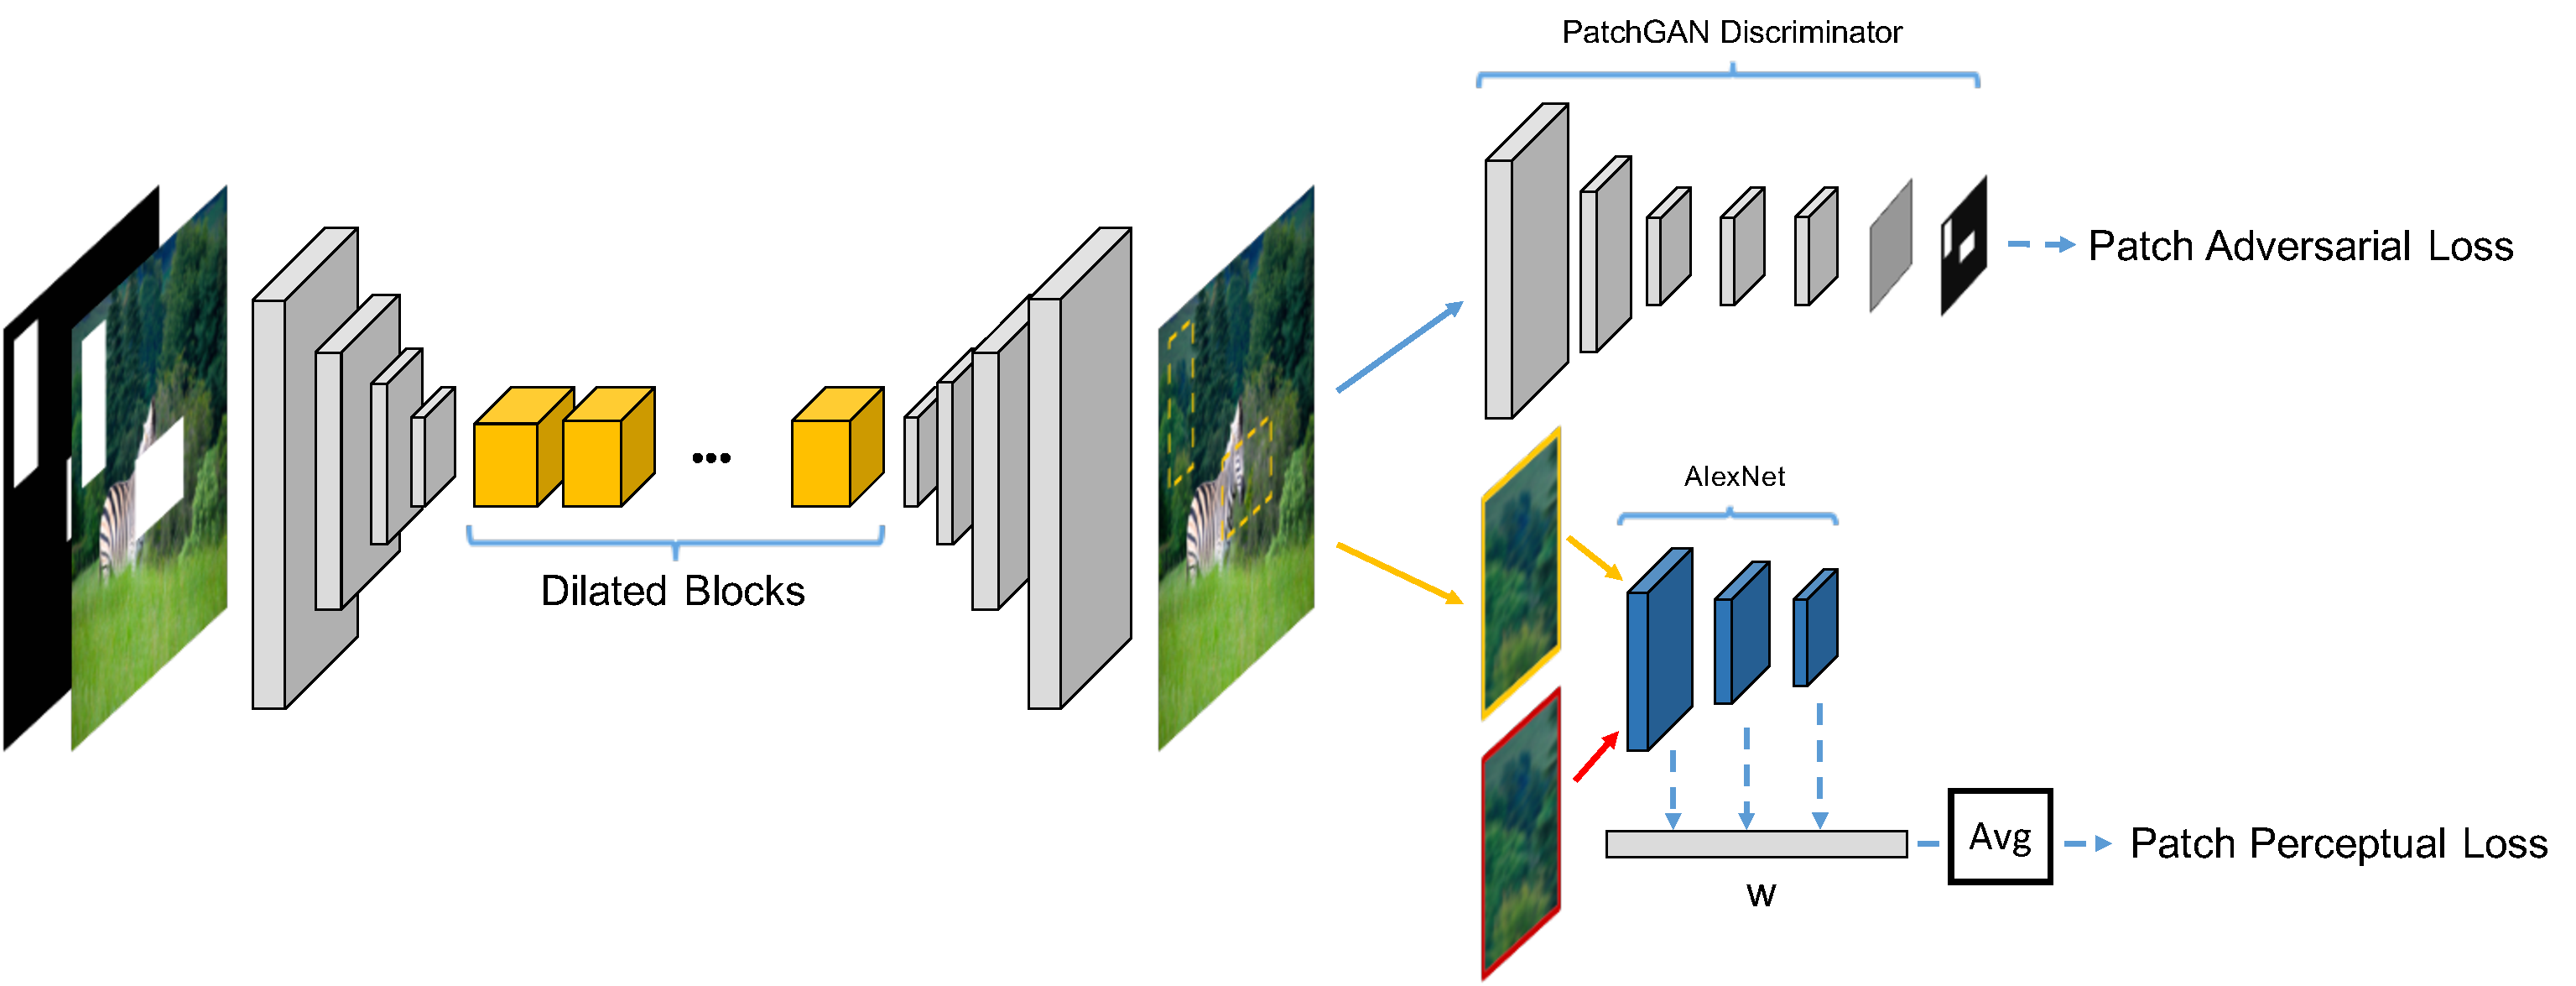
\includegraphics[width=1\textwidth]{figures/arch.pdf}
\caption{Generator head and the training losses. We only illustrate one scale of Patch Adversarial Loss and Patch Perceptual Loss. Note that to compute the Patch Adversarial Loss, we need to use the mask to find out which patch overlaps with the hole.}
\label{fig:model}
\vspace{-10pt}
\end{figure}

\subsection{The Generator Head}
\label{sec:resnet_head}

Previous research experimented with different architecture of $G$, most notably the U-Net style generator of~\cite{pathak2016context} and the FCN style generator of~\cite{iizuka2017globally}. ~\cite{iizuka2017globally} shows that FCN style inpainting network produces less blurred results than U-Net, as it adopts fully convolutional layers instead of an intermediate fully connected (FC) layer, which avoids significant resolution reduction or information loss. 

Similar to~\cite{iizuka2017globally}, our generator head is based on FCN and leverage the many properties of convolutional neural networks, including translation invariance and parameter sharing. Nevertheless, a major limitation of FCN is the constraint of the receptive field size, since the convolution layers are locally connected, making pixels far away from the hole carry no influence on the predicted hole content. We rely on several strategies to alleviate such drawback. First, like~\cite{iizuka2017globally}, we use a down-sampling front end to reduce the feature size, followed by multiple residual blocks~\cite{he2016deep}, and then an up-sampling back end to restore the full dimension. By downsampling, we increase the receptive field of the ResNet blocks. Second, we stack multiple ResNet blocks to further enlarge the receptive field. Finally, we adopt the dilated convolutional layers~\cite{yu2015multi} in all ResNet blocks. Dilated convolutions use spaced kernels, making it compute each output value with a wider view of input without increasing the number of parameters and computational burden. We set the dilation factor to 2 in all layers. Overall, we observe context is critical for realism, and the receptive size poses as an important factor for inpainting quality. This differentiates it from other image translation tasks. 

Specific to our network, the down-sampling front end consists of three convolutional layers, each with stride 2. The intermediate residual blocks contain 9 blocks stacked together, and the up-sampling back-end consists of three transposed convolution of stride 2. Each convolutional layer is followed by batch normalization (BN) and ReLu as the activation layer, except for the last layer which outputs the image. For down-sampling and up-sampling, an alternative would be using interpolated convolution to reduce the checkerboard effect, as suggested by~\cite{odena2016deconvolution}. The interpolated convolution uses a dimension-preserving convolution layer of stride 1, followed by max pooling or bilinear up-sampling. However, we observed that using interpolated convolution creates overly smooth effects. A detailed ablation study is presented in Sec.~\ref{sec:results}.

\subsection{The Training Losses}
Different losses have been used to train an inpainting network. These losses can be cast into two categories. The first category, which can be referred to as \textit{similarity loss}, is used to measure the similarity between the output and the original image. The second category, which we refer to as the \textit{realism loss}, is used to measure how realistic-looking the output image is. We summarize the losses used in different approaches in Table~\ref{table:losses}. 

\begin{table}[h!]
\begin{center}

\resizebox{1\textwidth}{!}{%
{\tiny
  \begin{tabular}{ l  c  c }
    \hline
    \textbf{Method} & \textbf{Similarity Loss} &  \textbf{Realism Loss} \\ \hline
    \emph{Context Encoder~\cite{pathak2016context}} & $\ell_2$ & Global Adversarial Loss\\ \hline
    \emph{Global Local Inpainting~\cite{iizuka2017globally}} & $\ell_2$ & Global and Local Adversarial Loss \\ \hline
    \emph{Our Approach} & Patch Perceptual Loss (PPL) & Improved Multi-Scale Adversarial Loss \\ \hline
    \hline
  \end{tabular}}
  }
  \end{center}
  \caption{Comparison of training losses in different methods.}
  \vspace{-10pt}
  \label{table:losses}
\end{table}

\noindent\textbf{Patch Perceptual Loss} As shown in Table~\ref{table:losses}, using $\ell_2$ loss for reconstruction and measure the disparity between the output and the original image has been the default choice of previous inpainting methods. However, it is known that $\ell_2$ loss does not correspond well to human perception of visual similarity (Zhang et al.~\cite{zhang2018unreasonable}). This is because $\ell_2$ losses wrongly assumes each output pixel is conditionally independent of all others. A well-known issue, for example, is that blurring an image leads to small changes in terms of Euclidean distance but causes significant perceptual difference. Recent research suggests that a better metric for perceptual similarity is the internal activations of deep convolutional networks, usually trained on a high-level image classification task. Such loss is called ``perceptual loss'', and is used in various tasks such as neural style transfer~\cite{gatys2016image}, image super-resolution~\cite{johnson2016perceptual}, and conditional image synthesis~\cite{dosovitskiy2016generating,chen2017photographic}.

Based on this observation, we propose a new ``patch perceptual loss'' as the substitute of the $\ell_2$ losses. Traditional perceptual loss typically uses VGG-Net, and computes the $\ell_2$ distance of the activations on a few feature layers. Recently,~\cite{zhang2016stackgan} specifically trained a patch perceptual network to measure the perceptual differences between two image patches based on AlexNet, making it an ideal candidate for our task. The patch perceptual network computes the activations across all feature layers and sums up the $\ell_2$ distances scaled by learned weights at each layer. Furthermore, to take into account both the local view and the global view of perceptual similarity, we compute PPL at two scales. Local PPL considers the local hole patch, while the global PPL slightly zooms out to cover a larger contextual area. More formally, our PPL is defined as:
\begin{eqnarray}
\sum\limits_{p=1,2}PPL_k(G(s)_p, x_p) = \sum\limits_{k=1,2}\sum\limits_l\frac{1}{H_lW_l}\sum\limits_{h,w}\parallel w_l^T\odot(\hat{F}(x_p)^l_{hw}-\hat{F}(G(s)_p)^k_{hw})\parallel^2_2.
\end{eqnarray}

Here $p$ refers to the hole patch. $\hat{F}$ is the AlexNet and $l$ is the feature layer. Abalation study in Sec.~\ref{sec:results} shows that PPL gives better inpainting quality than both $\ell_2$ and VGG-based perceptual losses. 

\noindent\textbf{Multi-Scale Patch Adversarial Loss} Adversarial losses are given by trained discriminators to discern whether an image is real or fake. The global adversarial loss of~\cite{pathak2016context} takes the entire image as input and outputs a single real/fake prediction, which does not consider the realism of local patches, especially the holes. The additional local adversarial loss of~\cite{iizuka2017globally} adds another discriminator specifically for the hole, but it requires the hole to be fixed shape and size during training to fit the discriminator. To consider both the global view and the local view, and to be able to use holes of arbitrary number and shapes, we propose to use PatchGAN discriminators~\cite{isola2016image} at three scales of image resolutions. The discriminator at each scale is identical, only the input is a differently scaled version of the \textit{entire image}. The PatchGAN discriminator at each scale is a convolutional discriminator which outputs a vector of predictions, where each value corresponds to an image patch. In this way, the discriminators are trained to classify global and local image patches across the image, and also enable us to use random holes and shapes during training. However, directly using PatchGAN is problematic in our case, as for the output restored image, only the patches overlapping with the hole area should be considered fake patches. Therefore when computing the discriminator loss of the restored image, instead of forcing the entire output to be fake, only the patches overlapping with the holes are labeled as fake. More formally, our Patch-wise Adversarial Loss is defined as: 
\begin{eqnarray}
\min\limits_G\max\limits_{D_1, D_2, D_3}&&\sum\limits_{k=1,2,3} L_{GAN}(G,D_k)  \\ = &&\sum\limits_{k=1,2,3}E_{(s_k,x_k)}[\log (s_k,x_k)] + E_s[\log (Q-D_k(s_k,G(s_k)))].
\end{eqnarray}
\label{eqn:adversarial_loss}
Here $k$ refers to the image scale, and $Q$ is a patch-wise real/fake vector, based on whether the patch overlaps with the holes. Using multiple GAN discriminators at the same or different image scale has been proposed in unconditional GANs~\cite{durugkar2016generative} and conditional GANs~\cite{wang2017high}. Here we extend the design to take into account inpainting hole locations, which is critical in obtaining semantically and locally coherent image completion results.

To summarize, our full objective combines both losses is therefore defined as:
\begin{eqnarray}
\min\limits_G((\max\limits_{D_1, D_2, D_3}\lambda_{Adv}\sum\limits_{k=1,2,3} L_{GAN}(G,D_k))+\lambda_{PPL}\sum\limits_{k=1,2}PPL_k(G(s)_p, x_p)).
\end{eqnarray}

We use $\lambda_{Adv}$ and $\lambda_{PPL}$ to controls the importance of the two terms. In our experiment, we set $\lambda_{Adv}=1$ and $\lambda_{PPL}=10$ to begin with. As training progresses, we gradually decrease the weight of $\lambda_{Adv}$ as explained in Sec.~\ref{sec:procedural}.

Fig.~\ref{fig:model} illustrates the architecture of our generator head and the training losses.

\subsection{Blockwise Procedural Training with Adversarial Loss Annealing}
\label{sec:procedural}
Our experiments show that using the described generator head and training losses already give inpainting results better than state-of-the-art. However, the results can still lack fine details, especially when synthesizing textures. Result may contain noise patterns when the image is complicated. A straight-forward effort to improve the results would be to stack more intermediate residual blocks to further expand the receptive view and increase the expressiveness of the model. However, we found that directly stacking more residual blocks makes it more difficult to stabilize the training. As the search space becomes much larger, it is also more challenging to find local optimum. In the end, the inpainting quality deteriorates as the model depth increases.

Recently, Progressive GAN~\cite{karras2017progressive} was proposed as a new training methodology for generative adversarial networks. The key idea is to grow both the generator and discriminator progressively, by adding new layers that model increasingly fine details as training progresses. This strategy makes the training faster and more stable and enables it to synthesize mega-pixel images with unprecedented visual quality.  

\begin{figure}[t]
\centering
\small
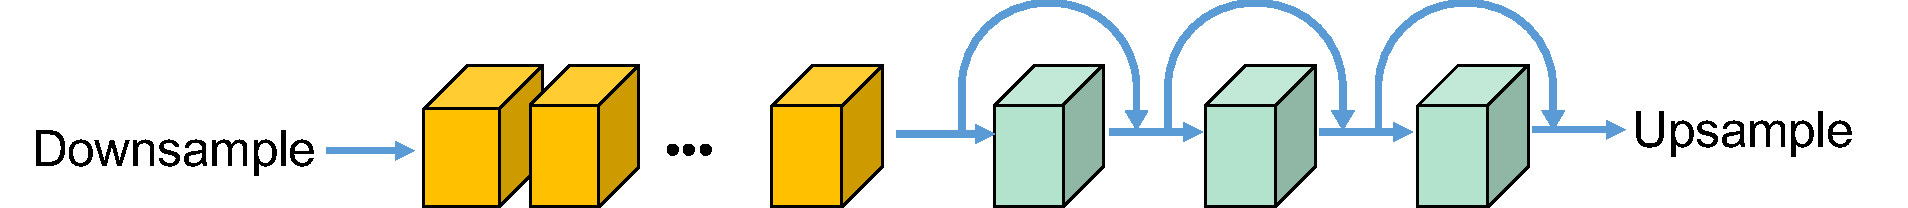
\includegraphics[width=1\textwidth]{figures/proc.pdf}
\caption{Illustration of block-wise procedural training. The yellow residual blocks refer to the generator head which are trained first. The green residual blocks are progressively added one at a time. We also draw the skip connections between the already trained residual blocks and the up-sampling back end.}
\label{fig:proc}
\vspace{-20pt}
\end{figure}

We adapt this idea for image inpanting and propose to use procedural block-wise training to gradually increase the depth of the inpainting network. More specifically, we begin by training the generator head until it converges. Then, we add a new residual block after the already trained residual blocks, right before the back-end upsampling layers. In order to smoothly introduce the new residual block without suddenly breaking the trained model, we add another skip path from the trained residual blocks to the upsampling layers. Initially, the weight of the skip path is set to 1, while the weight of the path containing the new block is set to 0. This essentially makes the initial network identical to the already trained network. We then slowly decrease the weight of the skip path and increase the weight of the new residual block as training progresses. In this way, the newly introduced residual block is trained to be a fine-tuning component, which adds another layer of fine details to the original results. This step are repeated multiple times, where each time we expand the model by adding a new residual block. In our experiment, we found that the results improve significantly after fine-tuning with the first additional residual block. The output becomes stabilized after three residual blocks, when little discernible changes can be detected if even more residual blocks are introduced. The procedural training process is illustrated in Fig.~\ref{fig:proc}.

We observe that the block-wise procedural training has several benefits. First, it guides the training process of a very deep generator. Starting with the generator head and gradually fine-tuning with more residual blocks makes it easier to discover the mapping between the incomplete image and the complete image, even though the search space is huge given the diversity of natural images and the random holes. Another benefit is reduced training time, as we found decoupling the training of the generator head and the fine-tuning of additional residual blocks requires significantly less training time comparing with training the network all at once.

\noindent\textbf{Adversarial Loss Annealing} During training, the generator adversarial loss updates the generator weight if the discriminator successfully detects the generated image as fake:
\begin{eqnarray}
\sum\limits_{k=1,2,3}E_s[\log (\bar{Q}-D_k(s_k,G(s_k)))].
\end{eqnarray}
Note that here $\bar{Q}$ reverses $Q$ of~\ref{eqn:adversarial_loss} as this is the loss to the generator. We observe that the generator adversarial loss becomes dominant over PPL as training progresses. This is because the discriminator becomes increasingly good at detecting fake images during training. This is less of a problem for image synthesis tasks. However, for the inpainting task which requires the output to be faithful to the original image, the outcome is that the generator deliberately adds noise patterns to confuse the discriminators, bringing more artifact to output or even synthesizing wrong textures. Based on this observation, we propose to use adversarial loss annealing, which decreases the weight of the generator adversarial loss when adding new residual block. More formally, let the initial weight of the generator adversarial loss be $\lambda^0_{adv}$, and the weight of the generator adversarial loss be $\lambda^i_{adv}$ after adding the $i_{th}$ residual block. We found that simply decay the weight linearly by setting $\lambda^i_{G_{adv}}=0.1^i\lambda^0_{G_{adv}}$ gives satisfying results. Detailed analysis are described in Sec.~\ref{sec:results}.

Finally, we summarize the discussed training schemes in Alg.~\ref{algo}.
\begin{algorithm}
\caption{Training the Inpainting Network}\label{algo}
\begin{algorithmic}[1]
\State Set batch size to 8 and basic learning rate to $lr_0\gets 0.0002$.
\State Set $\lambda_{PPL}\gets 10$ and $\lambda^0_{{adv}}\gets 1$.
\State Train the Generator Head $G_0$ using MSPAL and PPL (\ref{eqn:adversarial_loss}) for 150,000 iterations.
\For{i=1 to 3}
\State Add the skip path and the residual block $r_i$.
\State Set $lr_i\gets 0.1^i lr_0$ and $\lambda^i_{G_{adv}}\gets 0.1^i\lambda^0_{G_{adv}}$.
\State Train the generator $G_3$ with the added $r_i$ for 1,500 iterations.
\EndFor
\State \textbf{return} $G_3$ 
\end{algorithmic}
\end{algorithm}
